\documentclass[12pt,a4paper]{article}
\usepackage[utf8]{inputenc}
\usepackage[spanish]{babel}
\usepackage[margin=0.5in, top=0.5in, bottom=0.5in]{geometry}
\usepackage{amsmath}
\usepackage{amsfonts}
\usepackage{amssymb}
\usepackage{hyperref}
\usepackage{graphicx}
\usepackage[shortlabels]{enumitem}
\newcommand{\p}{\phantom{......}}

\title{Bases de datos 2023-1\\
Práctica 1: Bitácora}
\begin{document}
\maketitle

\textbf{Reporte de instalación:}\\
\begin{enumerate}
	\item \textit{Sistema operativo y versión:} GNU\\linux 5.19.5-zen (zen kernel)\\

	\item \textit{Distribución:} Arch linux\\

	\item \textit{Versión de la instalación:} psql (PostgreSQL) 14.5\\

	\item \textit{Tiempo requerido:} 15min\\

	\item \textit{Paso a Paso:}\\
		Primero busqúe los paquetes correspondientes en los repos de
		arch.Me tuve que asegurar de que \texttt{postgresql-contrib}
		no era necesario para la instalación.

		Luego actualize el sistema:\\
		\texttt{sudo pacman -Syu}\\
		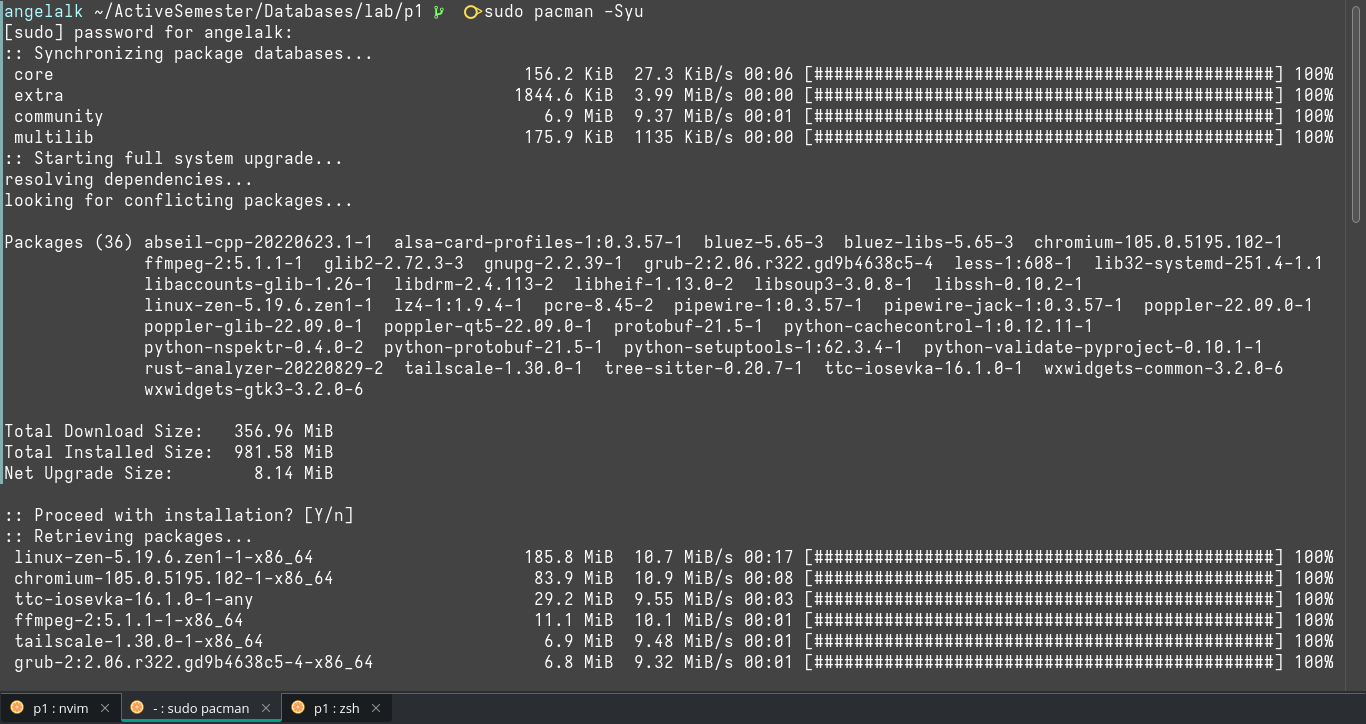
\includegraphics[scale=0.3]{assets/01-angel.png}

		Instalé los paquetes:\\
		\texttt{sudo pacman -S postgresql pgadmin4}\\
		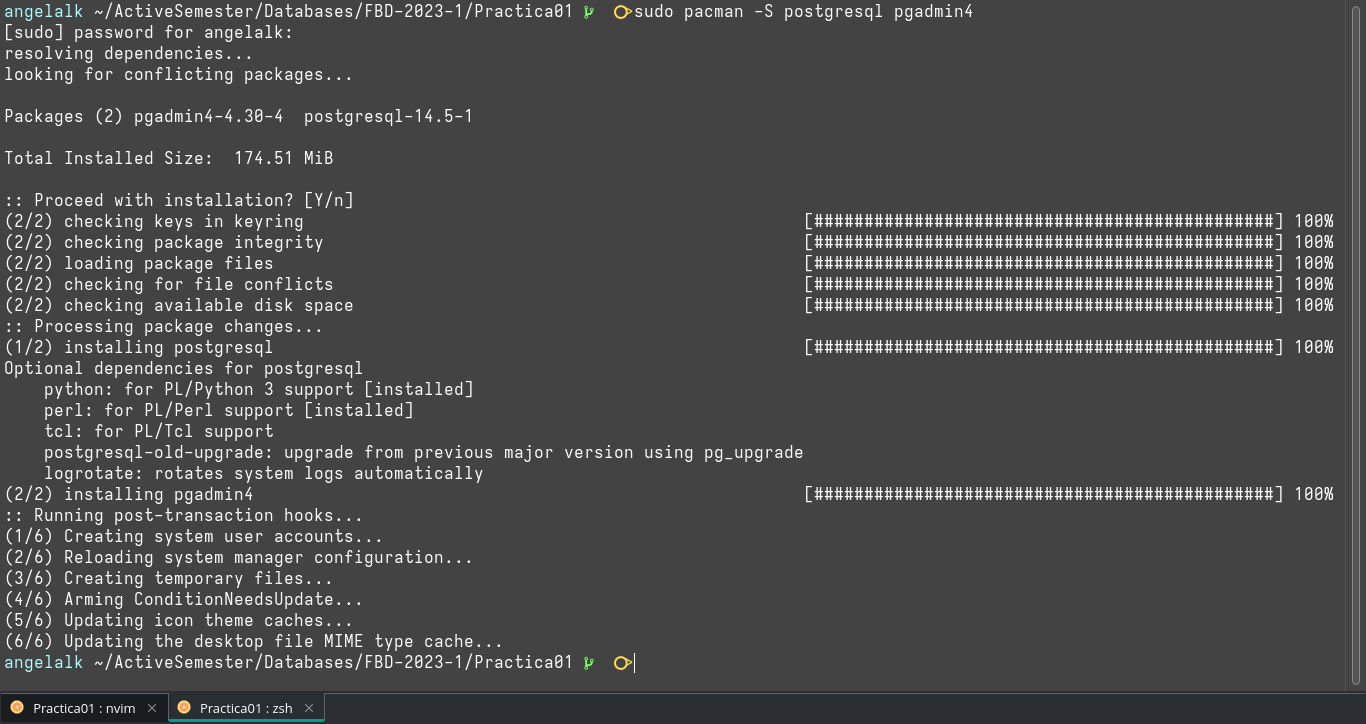
\includegraphics[scale=0.3]{assets/02-angel.png}

		Cambiar a usario de postgres:\\
		\texttt{sudo -iu postgres}\\

		Comando para iniciar cluster de postgress:\\
		\texttt{initdb -D /var/lib/postgres/data}\\
		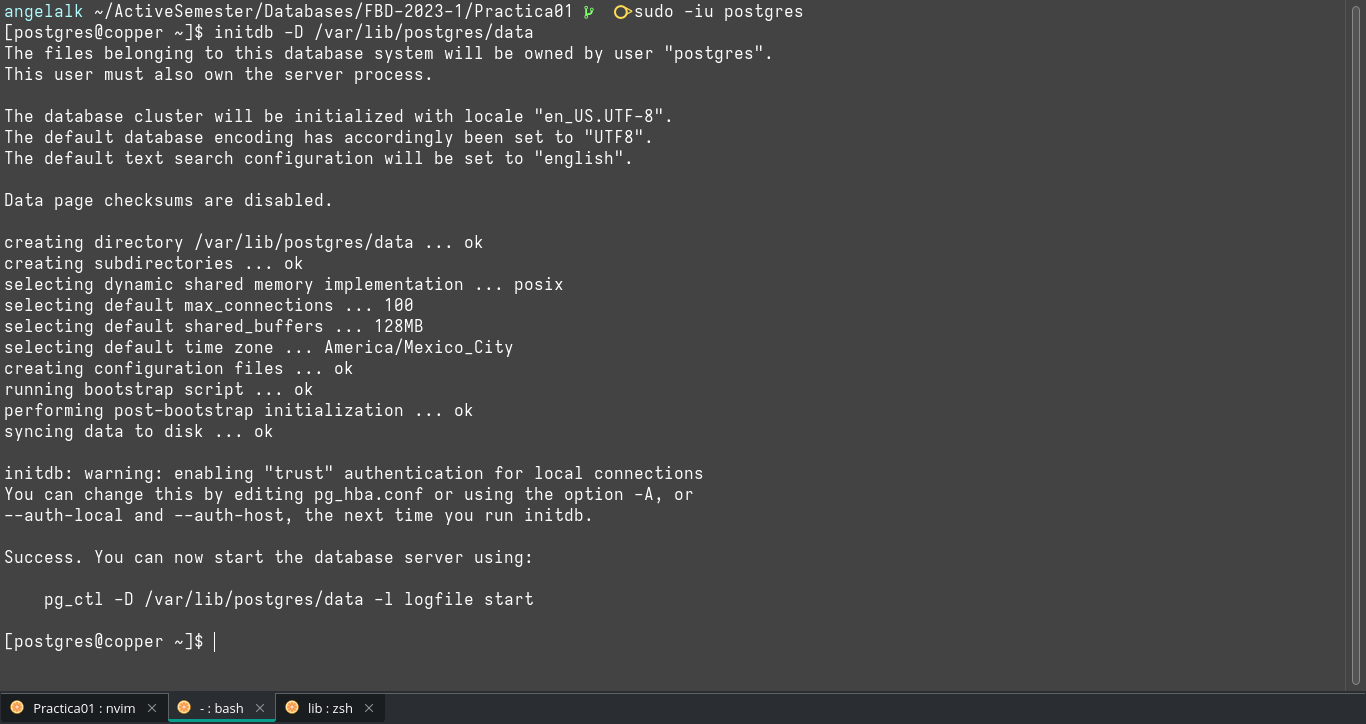
\includegraphics[scale=0.3]{assets/03-angel.png}

		Activamos el servicio de postgress:\\
		\texttt{sudo systemctl enable --now postgresql.service}\\
		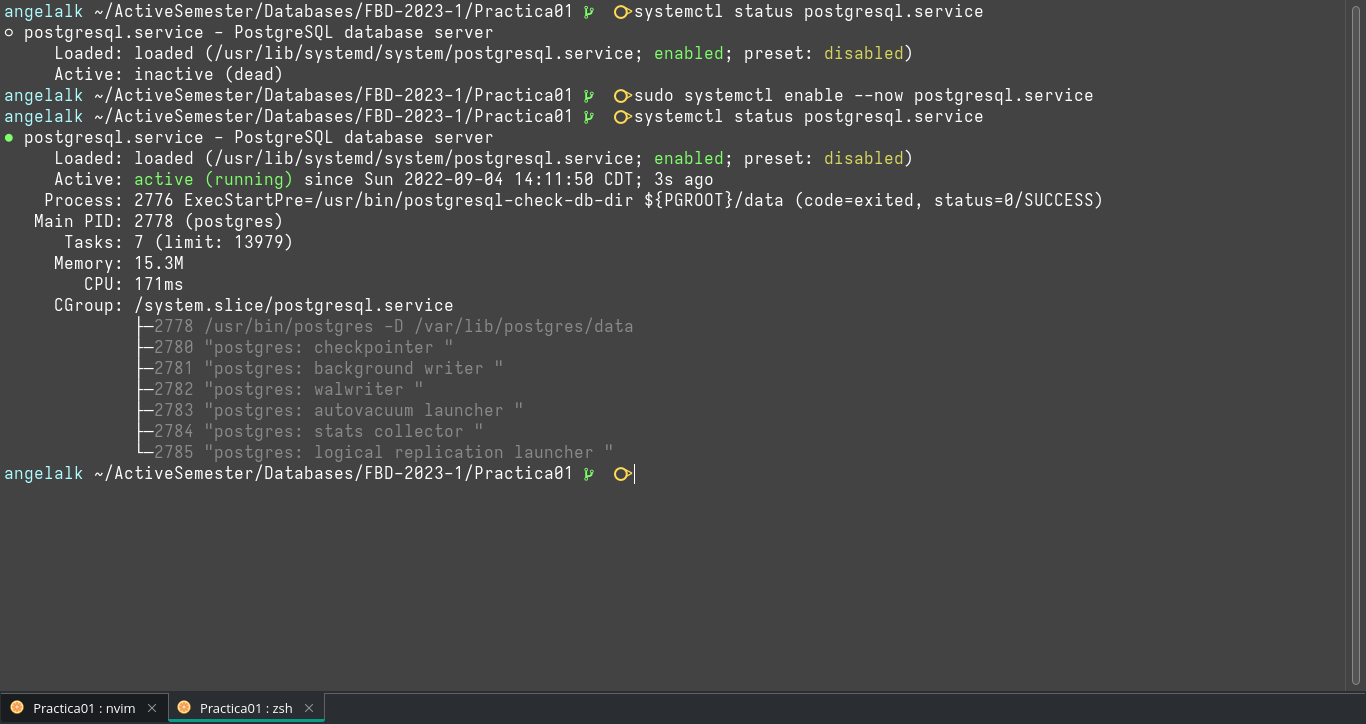
\includegraphics[scale=0.3]{assets/04-angel.png}

		Desde el usuario de postgress entramos al cliente y cambiamos la contraseña:\\
		\texttt{psql}\\
		\texttt{ALTER USER postgres WITH PASSWORD 'notmyrealpassword';}\\


	\item \textit{Comentarios y problemas:}\\
		El paquete \texttt{postgresql-contrib} no tiene equivalente en Arch,
		al parecer lo que tiene ya lo satisface el paquete de postgres.\\

		En Arch tienes que correr un comando para iniciar el cluster y luego
		activar el servicio de postgres, casi me equivoco.\\
\end{enumerate}

\end{document}
